\documentclass[journal]{vgtc}                % final (journal style)
%\documentclass[review,journal]{vgtc}         % review (journal style)
%\documentclass[widereview]{vgtc}             % wide-spaced review
%\documentclass[preprint,journal]{vgtc}       % preprint (journal style)

%% Uncomment one of the lines above depending on where your paper is
%% in the conference process. ``review'' and ``widereview'' are for review
%% submission, ``preprint'' is for pre-publication, and the final version
%% doesn't use a specific qualifier.

%% Please use one of the ``review'' options in combination with the
%% assigned online id (see below) ONLY if your paper uses a double blind
%% review process. Some conferences, like IEEE Vis and InfoVis, have NOT
%% in the past.

%% Please note that the use of figures other than the optional teaser is not permitted on the first page
%% of the journal version.  Figures should begin on the second page and be
%% in CMYK or Grey scale format, otherwise, colour shifting may occur
%% during the printing process.  Papers submitted with figures other than the optional teaser on the
%% first page will be refused.

%% These few lines make a distinction between latex and pdflatex calls and they
%% bring in essential packages for graphics and font handling.
%% Note that due to the \DeclareGraphicsExtensions{} call it is no longer necessary
%% to provide the the path and extension of a graphics file:
%% 
\includegraphics{diamondrule} is completely sufficient.
%%
\ifpdf%                                % if we use pdflatex
  \pdfoutput=1\relax                   % create PDFs from pdfLaTeX
  \pdfcompresslevel=9                  % PDF Compression
  \pdfoptionpdfminorversion=7          % create PDF 1.7
  \ExecuteOptions{pdftex}
  \usepackage{graphicx}                % allow us to embed graphics files
  \DeclareGraphicsExtensions{.pdf,.png,.jpg,.jpeg} % for pdflatex we expect .pdf, .png, or .jpg files
\else%                                 % else we use pure latex
  \ExecuteOptions{dvips}
  \usepackage{graphicx}                % allow us to embed graphics files
  \DeclareGraphicsExtensions{.eps}     % for pure latex we expect eps files
\fi%

%% it is recomended to use ``\autoref{sec:bla}'' instead of ``Fig.~\ref{sec:bla}''
\graphicspath{{figures/}{pictures/}{images/}{./}} % where to search for the images

\usepackage{microtype}                 % use micro-typography (slightly more compact, better to read)
\PassOptionsToPackage{warn}{textcomp}  % to address font issues with \textrightarrow
\usepackage{textcomp}                  % use better special symbols
\usepackage{mathptmx}                  % use matching math font
\usepackage{times}                     % we use Times as the main font
\renewcommand*\ttdefault{txtt}         % a nicer typewriter font
\usepackage{cite}
%% We encourage the use of mathptmx for consistent usage of times font
%% throughout the proceedings. However, if you encounter conflicts
%% with other math-related packages, you may want to disable it.

%% In preprint mode you may define your own headline.
%\preprinttext{To appear in IEEE Transactions on Visualization and Computer Graphics.}

%% If you are submitting a paper to a conference for review with a double
%% blind reviewing process, please replace the value ``0'' below with your
%% OnlineID. Otherwise, you may safely leave it at ``0''.
\onlineid{0}

%% declare the category of your paper, only shown in review mode
\vgtccategory{Research}

%% Paper title.
\title{Protein-Protein Interaction Interactive Exploration}

%% This is how authors are specified in the journal style

%% indicate IEEE Member or Student Member in form indicated below
\author{Katar\'{i}na Furmanov\'{a}, Kate\v{r}ina Kratochv\'{i}lov\'{a}, Jan By\v{s}ka, Ivan Viola, Eduard M. Gr\"{o}ller, Barbora Kozl\'{i}kov\'{a}}
\authorfooter{
%% insert punctuation at end of each item
\item
 Katar\'{i}na Furmanov\'{a} is with Masaryk University, Czech Republic. E-mail: furmanova@mail.muni.cz.
\item
 Kate\v{r}ina Kratochv\'{i}lov\'{a} is with Masaryk University, Czech Republic. E-mail: 374486@mail.muni.cz.
\item
 Jan By\v{s}ka is with Masaryk University, Czech Republic. E-mail: xbyska@fi.muni.cz.
\item 
Eduard M. Gr\"{o}ller is with TU Wien, Austria. Email: groeller@cg.tuwien.ac.at.
\item
Ivan Viola is with TU Wien, Austria. Email: viola@cg.tuwien.ac.at.
\item
Barbora Kozl\'{i}kov\'{a} is with Masaryk University, Czech Republic. E-mail: kozlikova@fi.muni.cz. 
}

%other entries to be set up for journal
\shortauthortitle{Furmanov\'{a} \MakeLowercase{\textit{et al.}}: Protein-Protein Interaction Interactive Exploration}
%\shortauthortitle{Firstauthor \MakeLowercase{\textit{et al.}}: Paper Title}

%% Abstract section.
\abstract{Studying the patterns of protein interactions is fundamental for understanding the structure and function of biological complexes. The exploration of the vast space of possible mutual conformations of interacting proteins and their contact zones is very time consuming and requires non-trivial user experience. Therefore, in this paper we propose three novel methods for guided exploration of the conformational space which help the domain experts to select the most biochemically relevant contact zones and explore them on different levels of detail. The first method, based on customized interactive heat maps, provides the overview of all possible protein conformations and their interactive filtering. The second method enables to traverse the pre-filtered conformations using a lens view. Here the conformation in focus is equipped with the information about interacting amino acids. These techniques are interactively linked with the third proposed method which represents individual conformations in three dimensional space. The problem of high overlaps of the conformations is solved by using exploded views equipped with 2D close-up views showing the details of the contact zone on different levels of abstraction. The usefulness of our methods was evaluated by the domain experts studying the structural maintenance of chromosomes.
} % end of abstract

%% Keywords that describe your work. Will show as 'Index Terms' in journal
%% please capitalize first letter and insert punctuation after last keyword
\keywords{Protein-protein interaction, heat plot, exploded view, contact zone.}

%% ACM Computing Classification System (CCS). 
%% See <http://www.acm.org/class/1998/> for details.
%% The ``\CCScat'' command takes four arguments.

\CCScatlist{ % not used in journal version
 \CCScat{I.3.6}{Picture/Image Generation}%
{Line and Curve Generation};
}

%% Uncomment below to include a teaser figure.
   \teaser{
   \centering
   
\includegraphics[width=16cm]{teaser.png}
   \caption{Visualization methods for exploration of conformations of protein-protein interactions. TODO change image and text.}
  }

%% Uncomment below to disable the manuscript note
%\renewcommand{\manuscriptnotetxt}{}

%% Copyright space is enabled by default as required by guidelines.
%% It is disabled by the 'review' option or via the following command:
% \nocopyrightspace

\vgtcinsertpkg

%%%%%%%%%%%%%%%%%%%%%%%%%%%%%%%%%%%%%%%%%%%%%%%%%%%%%%%%%%%%%%%%
%%%%%%%%%%%%%%%%%%%%%% START OF THE PAPER %%%%%%%%%%%%%%%%%%%%%%
%%%%%%%%%%%%%%%%%%%%%%%%%%%%%%%%%%%%%%%%%%%%%%%%%%%%%%%%%%%%%%%%%

\begin{document}

%% The ``\maketitle'' command must be the first command after the
%% ``\begin{document}'' command. It prepares and prints the title block.

%% the only exception to this rule is the \firstsection command
\firstsection{Introduction}

\maketitle
Understanding the constitution and biological function of proteins is essential in many research disciplines, namely in medicine and pharmaceutics.
This knowledge is tightly connected with the ability of the protein to interact with other molecules.
Proteins can interact with small molecules, called ligands, which enter the protein.
This process, called protein-ligand docking, is widely used in protein engineering where the goal is to change specific properties of a given protein by performing a chemical reaction between the protein and a ligand.
In drug design, the protein serves as a "factory" for ligand structural changes caused again by a mutual chemical reaction. 
Such modified ligand can then serve as a basis of a new drug. 
However, in drug design also the interactions between proteins are attracting increasing attention because most of the proteins critical for cellular life act in a cooperative manner forming multiprotein complexes. 
It is estimated that about 800 complexes exist in just one yeast cell. 
And all complexes are composed of subunits which constitute the complex via protein-protein interactions.
The main goal of the process of studying such protein-protein interactions, known as protein-protein docking, is to identify an appropriate spatial conformation of interacting proteins.
This requires the investigation and understanding of the mechanisms of the interactions and the identification of so called "hot spot" amino acids forming the contact zones between the interacting proteins.

Structure-determination of protein-protein interactions in laboratories is very challenging and time and money consuming, because of many problems related to the dynamic nature of the proteins, the difficulties with their purification and preparation of samples.
Therefore, computational docking helping with early understanding of the feasibility of proposed conformations between interacting proteins is currently very promising option and many algorithms and tools appeared in the last years.
The categorization of the existing algorithms along with the description of their basic principles was published recently by Huang~\cite{Huang2014}.
However, these tools are producing a large number of possible conformations and the domain expert has to explore them and select the most biochemically relevant ones. 
Therefore, the next step is to enhance the exploration process by other computational of visual support.
There were already several algorithms published for re-ranking of the conformations according to different criteria thus suggesting the user those conformations which should be explored in detail.
As a representative of these attempts, Malhotra et al.~\cite{Malhotra2015} in 2015 presented DockScore, a webserver for ranking the individual conformations produced by the docking tools. 
Their idea is based on building a scoring scheme considering several interface parameters, such as surface area, hydrophobicity, spatial clustering, etc.
This helps the user to reduce the amount of conformations to a smaller set which still has to be explored manually.
For this exploration the visual support is essential, enabling to see the spatial orientation of the contact zones and hot spot amino acids and to compare different conformations.
Figure~\ref{fig:dockscore} shows the existing visual representation of two different conformations which uses the combination of traditionally used techniques, cartoon and balls\&sticks.
The green and yellow proteins represent two different docking solutions with respect to the violet protein. 
Red and blue amino acids illustrate individual hot spot amino acids of the two corresponding contact zones.

\begin{figure}[bt]
  \centering
  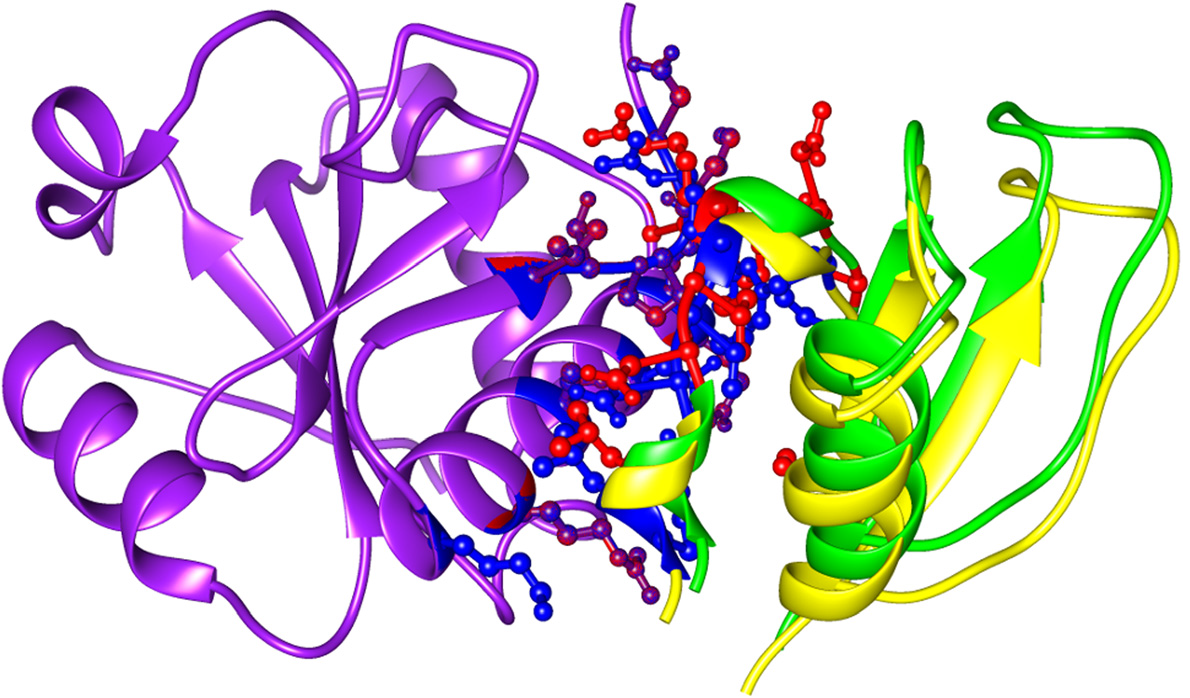
\includegraphics[width=1.0\columnwidth]{dockscore.png}
  \caption{Visual representation of the native and computed conformations of the protein complex with PDB ID 1SYX. Image taken from~\cite{Malhotra2015}.}
  \label{fig:dockscore}
\end{figure}

It is clearly visible that even for the comparison of two conformations the traditional representation suffers from many occlusion problems and it is hard to perceive the differences between individual solutions.
When comparing more conformations, even without detailed visualization of hot spot amino acids, the problem becomes even more visible (see Figure~\ref{fig:problem}).

\begin{figure}[bt]
  \centering
  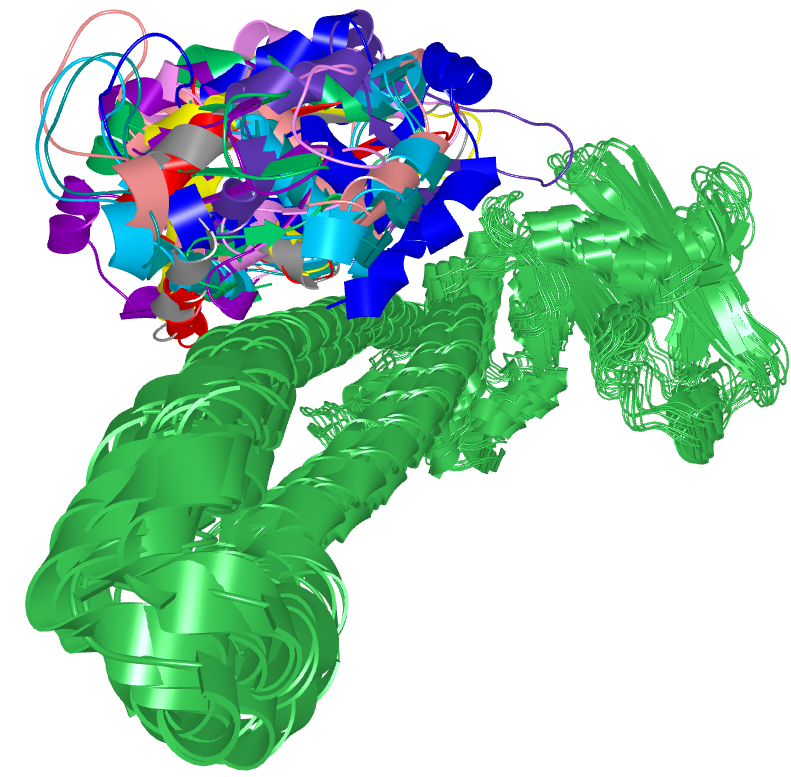
\includegraphics[width=0.7\columnwidth]{problem.png}
  \caption{Superimposition of several possible conformations between two proteins visualized using a traditional cartoon method. The set of green protein instances corresponds to one of
the interacting proteins, the colored components represent the second protein in different conformations.}
  \label{fig:problem}
\end{figure}

Therefore, in this paper we are proposing a solution to this problem.
We present three novel methods for visualization and comparison of individual conformations which aim to remove the problems of the existing solution and provide the domain experts with an intuitive and user friendly tool for interactive exploration of protein-protein interactions proposed by the computational tools.
Our solution is designed for dealing with large number of conformations so the user is not forced to use any of the re-ranking algorithms before using our solution. 

\section{Related Work}
In this section we will review the existing techniques related to our proposed representations of protein-protein interactions.
The problem of visual representation can be taken from different views.
One group of the existing solutions focuses on the visualization of whole networks of interacting proteins.
Because of their complexity, i.e., the number of interacting proteins, the visualizations are mostly graph-based.
Jeanquartier et al.~\cite{Jeanquartier2015} presented a survey of databases enabling the visual analysis of protein networks.

Second group consists of techniques visualizing the contact zones and their interacting amino acids.
The spatial techniques have to deal with the problem of occlusion and visual clutter caused by the fact that the most interesting parts of the interacting proteins, the contact zones, are positioned close to each other (see Figure~\ref{fig:varshney}a).
In other words, without any transformation or a visual enhancement (e.g., transparency) it is impossible to visually explore the contact zones.
Therefore, Jin et al.~\cite{Jin2014} presented the open-book view where the interacting proteins are rotated to face the contact zones towards the camera.
An alternative approach presented by Lee and Varshney~\cite{Varshney2003} computes and visualizes the intermolecular negative volume and the area of the docking site (Figure~\ref{fig:varshney}b,c).
This way the users can observe the volume between the interacting proteins without direct visualization of the contact zones themselves.
It can serve the domain experts as an interactive tool for studying possible docking conformations.

\begin{figure}[bt]
  \centering
  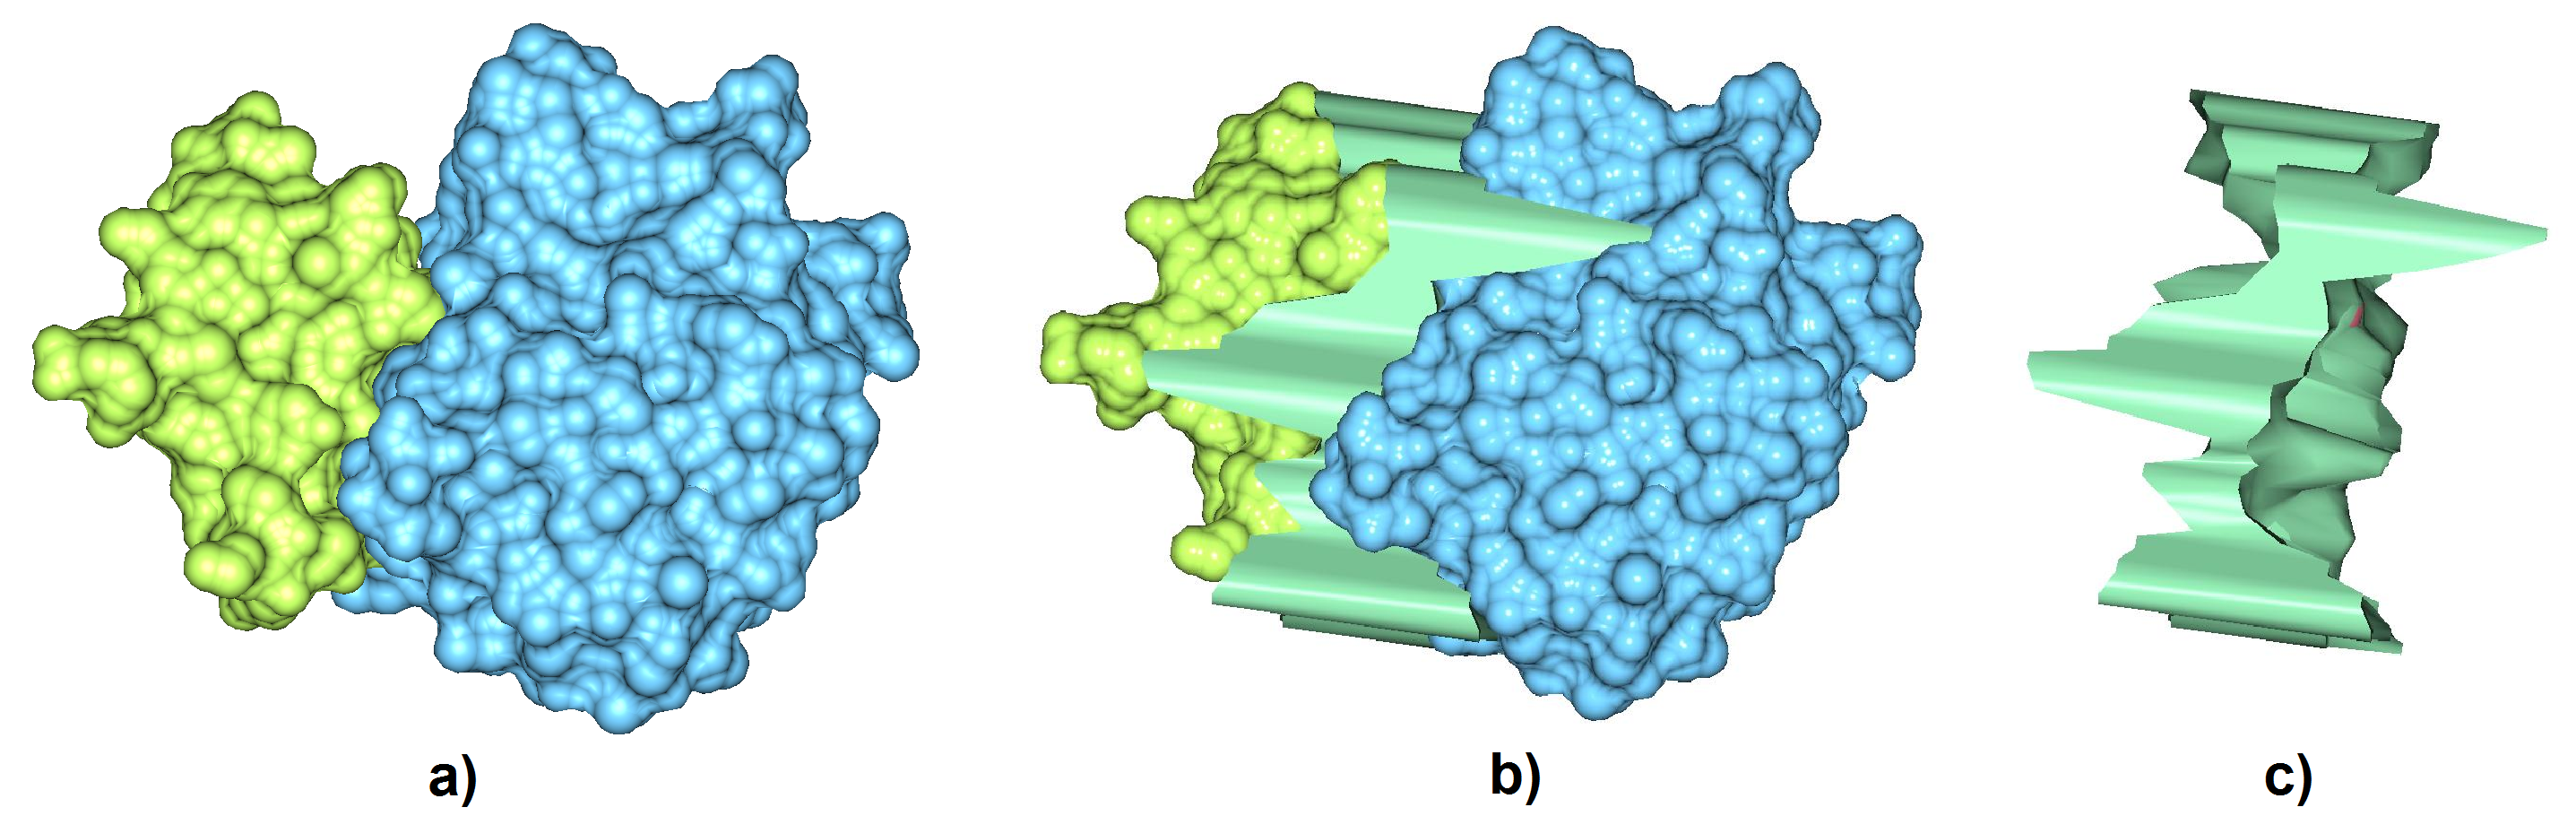
\includegraphics[width=1.0\columnwidth]{varshney.png}
  \caption{(a) Surface visualization of two interacting proteins with PDB ID 4SGB where the contact zones are not visible. (b) and (c) Visualization of the intermolecular negative surface representing the volume between the contact zones. Image taken from~\cite{Varshney2003}.}
  \label{fig:varshney}
\end{figure}

Alternative approaches to the visualization of contact zones can use abstracted 2D representations.
As an example of such approach can be taken the schematic representation of the contact zones used in the PDBsum database~\cite{pdbsum} which uses the overview visualization representing each of the interacting proteins by a sphere equipped with the information about the number of amino acids forming the contact zones and the number of different types of interactions between them.
Second visualization lists all contact zone amino acids. 
The interactions are visualized by lines of different colors and thickness which represent the type and strength of the interaction.

TODO some other list views??

matrices??

\section{Overview}


\section{Matrix View}

\section{Lens View}

\section{Exploded Views with Details on Contact Zones}

\section{User Interaction}

\section{Demonstration and Results}

\section{Conclusion}

%% if specified like this the section will be committed in review mode
%\acknowledgments{
%The authors wish to thank A, B, C. This work was supported in part by
%a grant from XYZ.}

%\bibliographystyle{abbrv}
\bibliographystyle{abbrv-doi}
%\bibliographystyle{abbrv-doi-narrow}
%\bibliographystyle{abbrv-doi-hyperref}
%\bibliographystyle{abbrv-doi-hyperref-narrow}
%%use following if all content of bibtex file should be shown
%\nocite{*}
\bibliography{template}
\end{document}

